% Document %
% Class %
\documentclass[12pt,twoside,onecolumn,a4paper]{article}

% Bibliography style %
%\usepackage[round]{natbib}

% Caption font to small and bold %
\usepackage[font=footnotesize,labelfont=bf,textfont=bf]{caption}

% Include figures %
\usepackage{graphicx}
\usepackage{float}
\usepackage{anyfontsize}
\usepackage{hyperref}
\usepackage{xcolor}
\usepackage{parskip}
\usepackage{./Functions/Palaeo}
\usepackage{./Functions/GECCO}

\usepackage{listings}
\lstset{language=Matlab,
          numbers=left,
          numberstyle=\footnotesize,
          xleftmargin=1cm,
          xrightmargin=1cm,
          backgroundcolor=\color{gray!35}}

% Define sub/section title format %
\usepackage[nobottomtitles]{titlesec}
\titleformat{\section}[block]{\vspace{-0.3cm} \bfseries}{\Large\thesection.}{1em}{\Large}[\vspace{-0.7cm}]
\titleformat{\subsection}[block]{\vspace{-0.1cm}\large\bfseries}{\thesubsection}{1em}{\large\vspace{-0.5cm}}
\titleformat{\subsubsection}[block]{\vspace{-0.3cm}\normalsize\bfseries}{\thesubsubsection}{1em}{\normalsize\vspace{-1cm}}

% Page Border %
\usepackage[inner=1.5cm,outer=1.5cm,top=1cm,bottom=1.8cm]{geometry}

% Remove Indent %
\setlength{\parindent}{0pt}

% Change font
\renewcommand*\rmdefault{lmss}

% Document %
\begin{document}

% Title and Author %
{
\centering
{\fontsize{25}{40}\selectfont \textbf{Documentation of the Geologically Evolving Carbon Cycle + Ocean model - GECCO}} \\[0.3cm]
{\Huge Ross Whiteford$^1$} \\ [0.2cm]
$^1$ School of Ocean and Earth Sciences, National Oceanography Centre Southampton, University of Southampton Waterfront Campus, European Way, Southampton, SO14 3ZH, UK
}

\begin{figure}[H]
\centering

\includegraphics[width=12cm]{./../Resources/Logo.png}
\end{figure}


\begin{figure}[H]
\centering
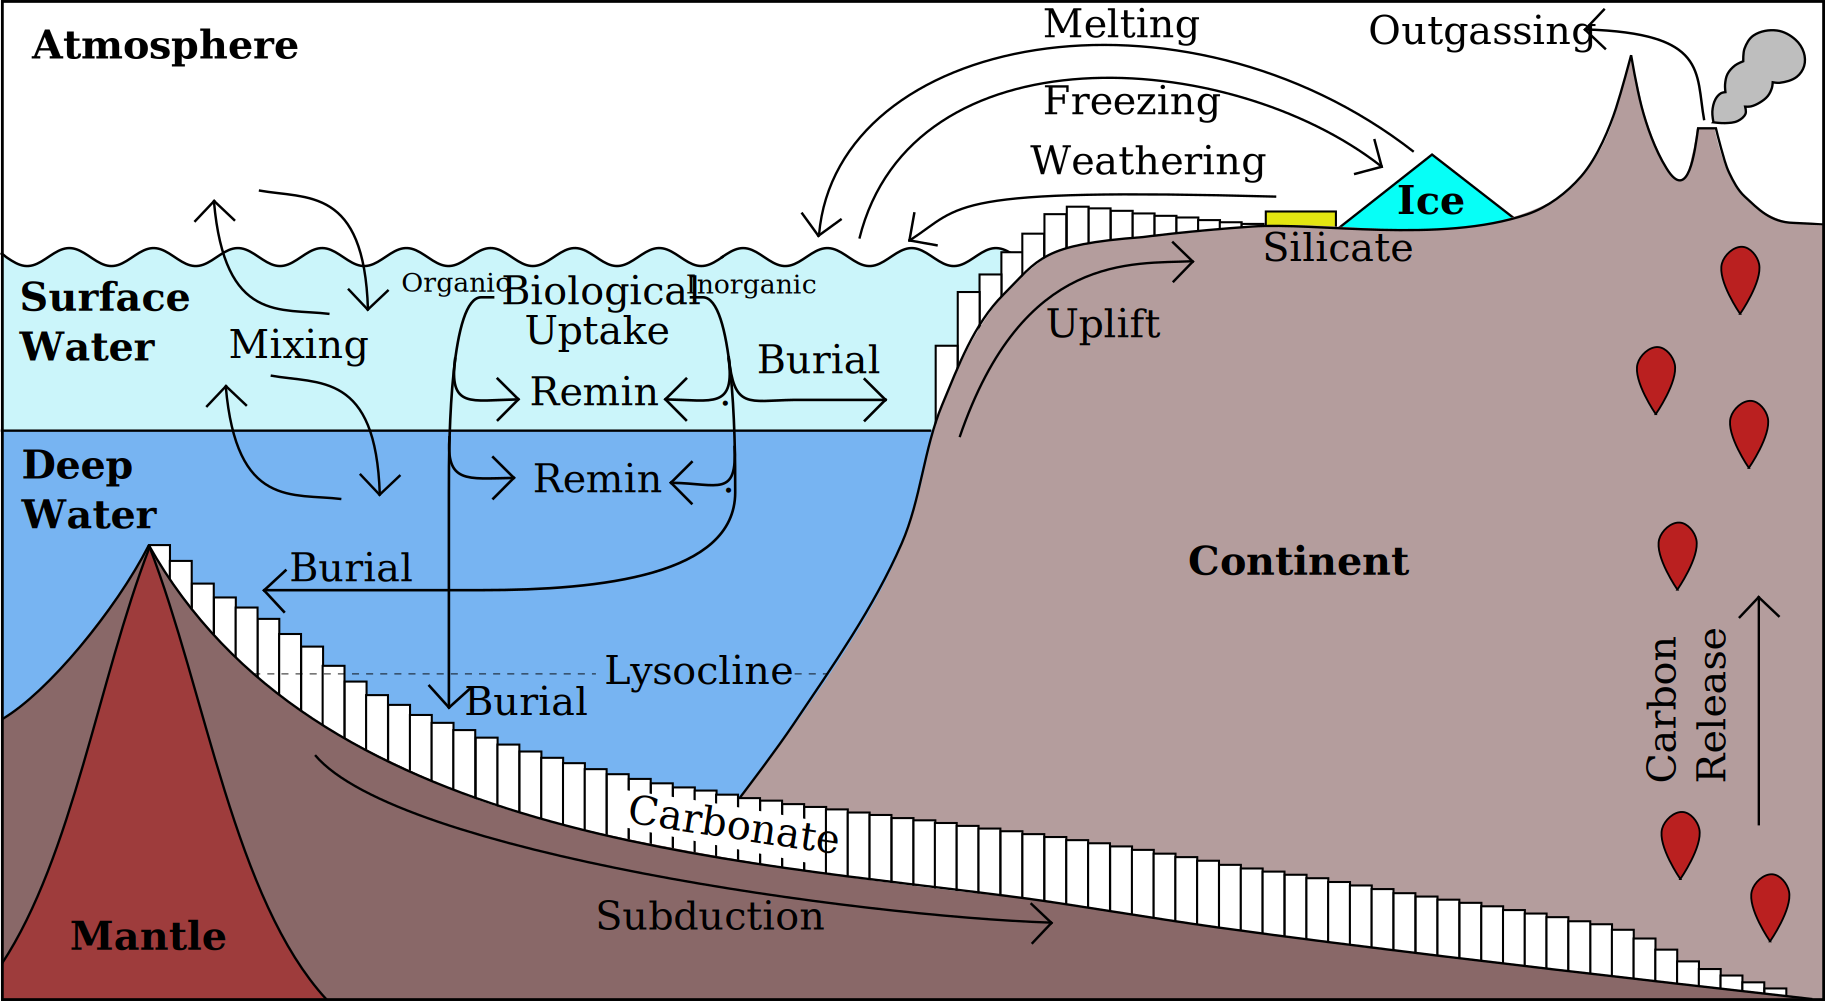
\includegraphics[width=18cm]{./../Resources/Model_Schematic.pdf}
\end{figure}
\clearpage

\raggedright
\raggedbottom
\section{Requirements}
\begin{enumerate}
\item GECCO v1.0.0 should work on any Windows computer using Matlab version 2016b and above.
\item GECCO v1.0.1 incorporates several bug fixes allows it to run on any Windows or Apple computer using Matlab version 2016b and above.
\end{enumerate}

\section{Source Code}
\labelSection{Source_Code}
Code releases can be found at: \href{https://github.com/Sciross/GECCO/releases}{https://github.com/Sciross/GECCO/releases}

The raw source code can be found at: \href{https://github.com/Sciross/GECCO/}{https://github.com/Sciross/GECCO/}

\section{Getting Started}
\subsection{Quickstart}
The easiest way to use GECCO is through the provided GUI. The GUI is not foolproof, and doesn't have the same flexibility as using GECCO directly, but should be sufficient for most use case scenarios.


\begin{figure}[H]
\centering
\includegraphics[width=10cm]{./Figures/Folder_Navigation.jpg}
\caption{Starting folder should be in Config}
\labelFigure{Folder_Navigation}
\end{figure}

To get started, ensure you have a copy of the code from the one of the sources listed in \refSection{Source_Code}. Open Matlab, and use the navigation pane to set the current working folder to the `Config' directory of the GECCO file structure (double click on the folder shown in \refFigure{Folder_Navigation}). Type this into the command prompt:
\begin{lstlisting}[language=Matlab]
Gui = GUI();
\end{lstlisting}

All being well, this should bring up the user interface splash page, with the logo, some filepath options, and some tickbox flags that looks vaguely like \refFigure{Splash_Page}.

\begin{figure}[H]
\centering
\includegraphics[width=15cm]{./Figures/Splash_Page.jpg}
\caption{Splash Page}
\labelFigure{Splash_Page}
\end{figure}

The flags along the bottom are, by default, set to save model results to file, but when these are active the model will not run unless there is an output filepath and filename specified - so for now, untick all the boxes. Then click on the `Run 1' tab along the top row.

\begin{figure}[H]
\centering
\includegraphics[width=15cm]{./Figures/Configuration_Page.jpg}
\caption{Configuration Page}
\labelFigure{Configuration_Page}
\end{figure}

This is the configuration page for GECCO. It should look something like \refFigure{Configuration_Page}. Without changing anything else, click the Run Model button (shown in \refFigure{Run_Model_Button}) once. 

\begin{figure}[H]
\centering
\includegraphics[width=10cm]{./Figures/Run_Model_Button.png}
\caption{Run Model Button}
\labelFigure{Run_Model_Button}
\end{figure}


Assuming you've changed the flags as described above, you should see the coloured square go from red to yellow, and the log box should read: \\
`Starting model runs...' \\
`Run number 1 of 1 starting @ HH:MM:SS' (with the appropriate time).

After a few minutes, the model run should complete. At this point, the square should turn from yellow to green, and the log box should read: \\
`Run number 1 of 1 complete @ HH:MM:SS' (with the appropriate time). \\
Successfully completed model runs!

If this isn't what happens, there's probably a bug. Please report it on the \href{https://github.com/Sciross/GECCO/}{GitHub repository}, and I can work on getting it sorted. Hopefully though, everything has gone well so far. If that's the case, try clicking on the `Plot Data' tab (at the top). This should show a series of subplots with time series of model results. Generally speaking these should be self explanatory, but for further details of each parameter will be added to this document as it evolves. As a rule of thumb, when there are two or more lines in a plot, light colours show surface ocean values and darker colours show deep ocean values - if there is a third line in a different colour this is typically the atmospheric value. The arrows at either side allow you to scroll through the subplots that are produced. Hopefully these are all self explanatory - but if you have questions, please raise them as an issue with the documentation using the \href{https://github.com/Sciross/GECCO/}{GitHub}, and I will add the information.

You are now able to run GECCO!

\subsection{A little more}
There are a quite a few ways of customising GECCO runs. The timing is controlled by the values in the table shown in \refFigure{Run_Table}. Internally, GECCO represents time as a series of contiguous \Chunks. \Chunks can be added and removed using the + and - sign adjacent to the \Chunks table, and can be loaded from file using the load button. The first three columns of the \Chunks table (`start', `end' and `step') control the timepoints at which the model calculation is run (by default from 0 to 1Myr, with a spacing of 20yr). The final three columns (`start', `end' and `step') control the timepoints at which model output is produced (by default from 0 to 1Myr, with a spacing of 100yr). The first two columns in the \Chunks table must create a contiguous time series (for example you may specify two \Chunks such as, 0-1Myr and 1-2Myr, but not 0-1Myr and 2-3Myr. Currently, the output resolution must be an integer multiple of the input resolution (e.g. 100yr is exactly five times 20yr).

\begin{figure}[H]
\centering
\includegraphics[width=10cm]{./Figures/Run_Table.jpg}
\caption{Run Table}
\labelFigure{Run_Table}
\end{figure}

The values used to control the parameters in GECCO are specified using the conditions table (\refFigure{Conditions_Table}). This operates using three dropdown menus that allow you to specify which values you would like to change. The \Initials and \Constants options control the initial conditions and constant conditions respectively. The \Functionals option allows you to choose some of the functions that control model behaviour. Simply select the appropriate words from the dropdown menus to choose a particular value, then edit the value in the table. For example, you can try changing the Initials->Atmosphere\_CO2 value to `1200e$-6$', then rerun the model to see the impact.

\begin{figure}[H]
\centering
\includegraphics[width=10cm]{./Figures/Conditions_Table.jpg}
\caption{Conditions Table}
\labelFigure{Conditions_Table}
\end{figure}

The final part of this introductory material is the so called Changes table. The Changes table allows users to make perturbations (instantaneous changes to model parameters that occur between \Chunks), and to define transients (long term changes that link one model parameter to another). To add a Change, select the appropriate category from the dropdown menu, then select the + button (and remove with the - button). Fill in the required values using the dropdown menus that are created, until the final column where text entry is required. In this case of a perturbation, the simplest example is to set the final column to a value (e.g. choose to perturb atmospheric \COTwo up to `1200e-6'). In the case of a transient, the simplest example is to set the final column to the variable `t' (which will make the chosen variable equal to the model time in years).


\section{Advanced Usage}
TBC

\end{document}